% Anonymous review manuscript. Compile with pdfLaTeX twice, or Tectonic.
% All tables, vector figures, and references are embedded in this file.
% The venue requests DOC/DOCX for submission: this LaTeX source is an authoring
% deliverable. Conversion to Word requires a separate layout/page-count check.
\documentclass[conference,a4paper,10pt]{IEEEtran}
\usepackage[T1]{fontenc}
\usepackage{newtxtext}
\usepackage[left=1.60cm,right=1.60cm,top=1.90cm,bottom=2.54cm]{geometry}
\usepackage{booktabs,tabularx,array}
\usepackage{graphicx}
\usepackage{tikz}
\usetikzlibrary{arrows.meta,positioning,fit,calc}
\usepackage[hidelinks,pdfauthor={},pdftitle={Evidence Guided Smart Contract Repair with Deterministic Execution Gates}]{hyperref}
\usepackage{url}
\setlength{\columnsep}{0.635cm}
\newcolumntype{Y}{>{\raggedright\arraybackslash}X}
\pagestyle{empty}
\raggedbottom
\newcommand{\code}[1]{\texttt{#1}}
\newcommand{\sys}{Sentinel}
\begin{document}
\title{Sentinel: An Evidence-Guided Multi-Agent Framework for Smart Contract Vulnerability Confirmation and Closed-Loop Remediation
}
\author{
\small
\begin{tabular}{@{}c@{\hspace{0.025\textwidth}}c@{\hspace{0.025\textwidth}}c@{}}
\parbox{0.29\textwidth}{\centering\textbf{Manjunath D. R.}\\[-0.2ex]\textit{Faculty Guide}\\[-0.2ex]\textit{Department of Computer Science and Engineering}\\\textit{IoT and Cybersecurity including Blockchain Technology}\\B.M.S. College of Engineering\\Bengaluru, India} &
\parbox{0.29\textwidth}{\centering\textbf{K R Pranav Swaroop Reddy}\\\textit{Department of Computer Science and Engineering}\\\textit{IoT and Cybersecurity including Blockchain Technology}\\B.M.S. College of Engineering\\Bengaluru, India} &
\parbox{0.29\textwidth}{\centering\textbf{Chinmay Hegde}\\\textit{Department of Computer Science and Engineering}\\\textit{IoT and Cybersecurity including Blockchain Technology}\\B.M.S. College of Engineering\\Bengaluru, India}\\[1.6em]
\multicolumn{3}{c}{\begin{tabular}{@{}c@{\hspace{0.06\textwidth}}c@{}}
\parbox{0.29\textwidth}{\centering\textbf{Jnan Dev B L}\\\textit{Department of Computer Science and Engineering}\\\textit{IoT and Cybersecurity including Blockchain Technology}\\B.M.S. College of Engineering\\Bengaluru, India} &
\parbox{0.29\textwidth}{\centering\textbf{Suhas P}\\\textit{Department of Computer Science and Engineering}\\\textit{IoT and Cybersecurity including Blockchain Technology}\\B.M.S. College of Engineering\\Bengaluru, India}
\end{tabular}}
\end{tabular}
}
\maketitle
\thispagestyle{empty}

\begin{abstract}
Smart contract analyzers identify suspicious code, but a warning alone does not show that an attacker can exploit the contract or that a proposed repair is safe. We present Sentinel, an evidence-guided workflow for Foundry projects. Scout normalizes and ranks static and symbolic findings; Red Team converts a selected finding into an executable proof-of-concept; Blue Team proposes a focused patch; and a deterministic Validator rebuilds the project, replays the exploit, and runs regression tests. A shared state ledger preserves source snapshots, tool diagnostics, generated artifacts, patch attempts, and final decisions. This separation prevents unconfirmed warnings from being presented as vulnerabilities and untested edits from being presented as repairs. We evaluate the implementation at two levels. All 82 automated tests passed in 6.16 seconds. In a declared four-fixture engineering benchmark, all four known vulnerabilities were exploited and all four template repairs passed build, exploit-defense, and regression gates, with zero retries and a mean end-to-end time of 31.226 seconds. These results validate the implemented fixture workflow, not general repair ability. Slither failed in all four benchmark runs and the dataset contains no clean controls; consequently, no case entered the detection-metric denominator and precision, recall, F1, and false-positive rate are not reported. The 500-project FORGE manifest remains an evaluation input rather than completed end-to-end evidence. Sentinel therefore contributes a reproducible integration framework and a transparent basis for a larger held-out evaluation.
\end{abstract}
\begin{IEEEkeywords}
smart contract security, automated program repair, executable exploits, static analysis, verification
\end{IEEEkeywords}

\section{Introduction}
Analyzer warnings do not prove exploitability, and compilable patches do not prove mitigation. Slither supplies structured Solidity findings, while hybrid tools such as MPro combine static and symbolic evidence~\cite{slither,mpro}. PoCo shows the value of executable Foundry proof-of-concept (PoC) tests, and repair research emphasizes both exploit mitigation and behavior preservation~\cite{poco,mitigation}. This motivates Sentinel: a Python workflow in which Scout ranks candidates, Red Team executes an exploit, Blue Team proposes a focused repair, and a deterministic Validator rebuilds and tests the result. Fixed demonstration templates keep the reviewed path inspectable.

This gap creates a practical burden for developers. Analyzer outputs use different schemas, severities, and source mappings; an apparent vulnerability may be unreachable in context; and a plausible edit may suppress an attack only by breaking intended functionality. Language models can help construct tests and patches, but textual confidence is not an execution oracle. A useful remediation workflow must preserve provenance, require observable attack impact, constrain source modification, and expose failed tools or gates instead of hiding them behind one score.

Sentinel addresses this problem as an evidence pipeline for local Foundry projects. Static and symbolic reports are normalized without discarding their origin. A selected candidate advances only after Forge executes a project-specific attack. The repair is applied to an isolated copy and accepted only after compilation, replay of the same exploit, and regression testing. A shared ledger supports both developer review and benchmark aggregation. When evidence is unavailable or contradictory, the workflow records the limitation rather than claiming that the contract is safe.

We ask whether candidates can be confirmed (\textbf{RQ1}), supplied attacks reproduce their impacts (\textbf{RQ2}), repairs block attacks while preserving tests (\textbf{RQ3}), retries recover rejected repairs (\textbf{RQ4}), and what cost is recorded (\textbf{RQ5}). This study answers RQ2, fixture-scoped RQ3, runtime and retries; held-out RQ1/RQ4 remain open. The contributions are: (1) an implemented workflow joining discovery, confirmation, repair, and validation; (2) a typed evidence ledger and guarded patch path; (3) a deterministic exploit-replay gate; and (4) an experiment runner with baseline and ablation profiles. Both successful execution and incomplete coverage are reported so the conclusions follow the available evidence.

\section{Background and Related Work}
\subsection{Analysis and Reproducible Tool Execution}
Slither supports dataflow and taint analysis, while MPro uses static evidence to guide symbolic exploration~\cite{slither,mpro}. Sentinel normalizes their outputs but retains tool, detector, and source identity. SmartBugs motivates reproducible tool execution~\cite{smartbugs}; Sentinel instead studies the transition from warning to executable confirmation and repair.

\subsection{Exploit Generation and Program Repair}
PoCo's reason--act--observe loop generates executable Foundry exploits~\cite{poco}. Sentinel extends this idea through repair and validation. Prompt to Pwn studies LLM exploit generation, while V2E emphasizes triggerability and observable impact~\cite{prompttopwn,v2e}.

SmartFix ranks generate-and-verify repairs; ContractTinker uses LLM repair with Foundry; and SCPatcher adds retrieved knowledge~\cite{smartfix,contracttinker,scpatcher}. Mitigation studies warn that passing one attack test does not prove full correctness~\cite{mitigation}. Echidna and ordering-aware fuzzing suggest future extensions beyond templates~\cite{echidna,fuzzordering}. Multi-agent surveys and LLM4Vuln further motivate separating generation, execution, and review~\cite{multise,llm4vuln}.

\subsection{Research Gap and Novelty}
Prior work often evaluates detection, exploitation, or repair separately~\cite{slither,poco,smartfix,contracttinker,scpatcher}. Sentinel connects these boundaries: Forge must confirm a candidate, and the same exploit plus regressions must validate its repair. The serialized transitions, failures, and retries form an inspectable integration and evaluation harness.

\section{Problem and Design Goals}
\subsection{Inputs and Scope}
Input is a local Foundry project; output is a reviewable patch with candidate, exploit, command, and validation evidence. Missing tools are reported as incomplete coverage, never as safety. Demonstrations cover reentrancy, missing access control, \code{tx.origin}, and unchecked calls. Other findings may use an optional model provider, but economic attacks, oracle manipulation, and arbitrary cross-contract invariants remain outside the demonstrated scope.

The problem is modeled as a sequence of evidence transformations. Given project $P$, the analyzers produce candidate set $C$. Scout selects candidate $c\in C$; Red Team seeks an executable test $e$ that demonstrates a security impact on $P$; Blue Team produces patch $p$ only after $e$ succeeds; and Validator evaluates $p(P)$ against compilation, exploit replay, and regression oracles. The workflow returns a verified repair only when all configured gates pass. Otherwise, it records an abstention, failure, or bounded retry. This formulation keeps detection confidence separate from exploit evidence and repair evidence.

\subsection{Design Requirements}
Five requirements guide the implementation: \textbf{evidence before escalation} retains provenance and requires an executed exploit; \textbf{deterministic acceptance} uses compilation and tests; \textbf{minimal mutation} confines edits to an isolated copy; \textbf{explicit incompleteness} records tool and parsing failures; and \textbf{reviewability} stores the PoC, diff, commands, retries, and outcome. Deployment decisions remain with the developer.

\subsection{Evidence Used by the Workflow}
Each candidate stores tool, detector, location, severity, explanation, and raw output. Red Team must demonstrate observable impact. Validator accepts a repair only when it compiles, blocks the confirmed exploit, and preserves remaining tests. These checks are reviewable but prove only the exercised behaviors.

The evidence has three levels. Analyzer output is \emph{candidate evidence}; a passing attack on the original project is \emph{confirmation evidence}; and a successful build, blocked attack, and passing regression suite are \emph{repair evidence}. Reports preserve these labels so that a user can distinguish discovered warnings, confirmed bugs, attempted changes, and accepted repairs. This distinction is also necessary for benchmarking because each level has a different denominator and failure mode.

\subsection{Trust Boundary}
The intended environment is a developer-controlled project. Source, analyzer descriptions, and model responses are untrusted inputs. Argument arrays, an executable allowlist, validated directories, and timeouts constrain commands, but do not create a security sandbox for hostile projects.

\section{System Architecture}
\subsection{Workflow and State Ledger}
Fig.~\ref{fig:architecture} presents the principal stages. A LangGraph state machine coordinates the workflow, while a Pydantic state model records source snapshots, analyzer runs, candidate selection, exploit artifacts, patch attempts, execution results, and retry history. JSON serialization makes the same record available to reporting and subsequent inspection. The ledger records observations; it is not a cryptographic attestation or an append-only audit service.

\begin{figure*}[t]
\centering
\resizebox{\textwidth}{!}{%
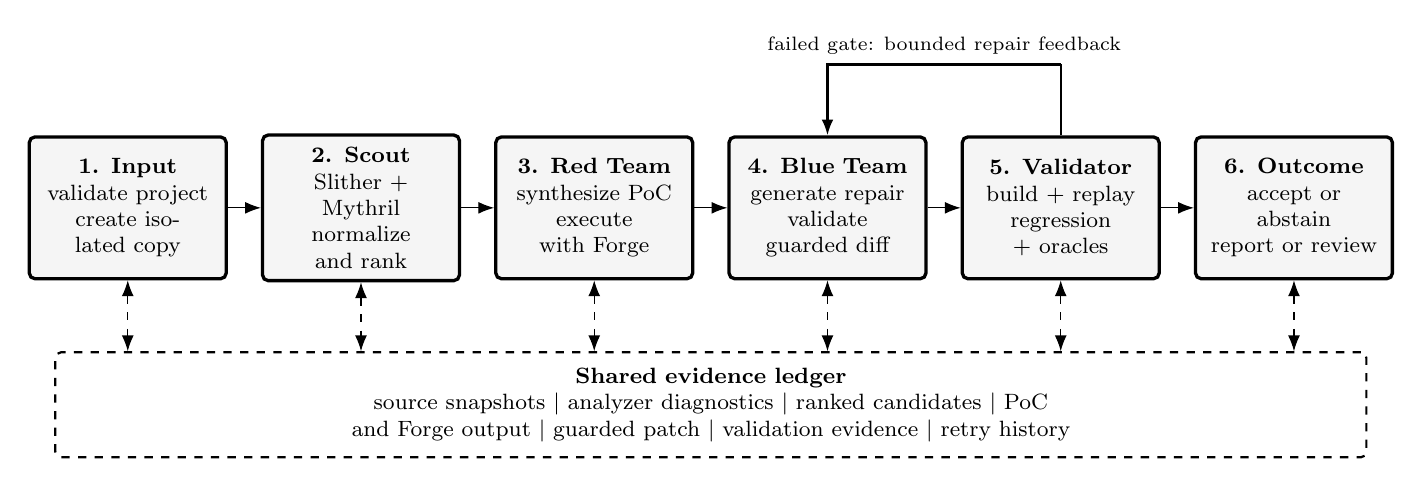
\begin{tikzpicture}[font=\footnotesize, node distance=4.2mm,
 stage/.style={draw,very thick,rounded corners=2pt,align=center,text width=2.18cm,minimum height=18mm,inner sep=1.6mm,fill=black!4},
 ledger/.style={draw,thick,dashed,rounded corners=2pt,align=center,text width=16.25cm,minimum height=10mm,inner sep=2mm},
 >={Latex[length=2mm]}]
\node[stage] (copy) {\textbf{1. Input}\\validate project\\create isolated copy};
\node[stage,right=of copy] (scout) {\textbf{2. Scout}\\Slither + Mythril\\normalize and rank};
\node[stage,right=of scout] (red) {\textbf{3. Red Team}\\synthesize PoC\\execute with Forge};
\node[stage,right=of red] (blue) {\textbf{4. Blue Team}\\generate repair\\validate guarded diff};
\node[stage,right=of blue] (judge) {\textbf{5. Validator}\\build + replay\\regression + oracles};
\node[stage,right=of judge] (report) {\textbf{6. Outcome}\\accept or abstain\\report or review};
\foreach \a/\b in {copy/scout,scout/red,red/blue,blue/judge,judge/report}
 \draw[->] (\a)--(\b);
\node[ledger,below=9mm of $(red.south)!0.5!(blue.south)$] (state) {\textbf{Shared evidence ledger}\\source snapshots $\mid$ analyzer diagnostics $\mid$ ranked candidates $\mid$ PoC and Forge output $\mid$ guarded patch $\mid$ validation evidence $\mid$ retry history};
\foreach \a in {copy,scout,red,blue,judge,report}
 \draw[<->,dashed] (\a.south)--(\a.south |- state.north);
\draw[thick] (judge.north) -- ++(0,9mm) coordinate (feedbacktop);
\draw[->,thick] (feedbacktop) -- node[above,font=\scriptsize]{failed gate: bounded repair feedback} (feedbacktop -| blue.north) -- (blue.north);
\end{tikzpicture}
}
\caption{Expanded Sentinel workflow. Solid arrows show control flow, dashed arrows show state exchange, and the feedback edge carries failed validation evidence into a bounded repair retry.}
\label{fig:architecture}
\end{figure*}

\subsection{Orchestration and Shared State}
Sentinel copies source, configuration, and tests into a temporary workspace, excluding caches and version-control data. LangGraph moves this copy through the four roles. A shared Pydantic state holds snapshots, analyzer output, the selected finding, exploit, patch, command results, retries, and final status; JSON serialization supports inspection and reproduction.

Each node returns a typed state update. Conditional edges route confirmed exploits to repair, rejected exploits to reporting, accepted patches to output, and failed validation to the bounded correction edge in Fig.~\ref{fig:architecture}. Only the disposable workspace receives generated tests and patches.

\subsection{Scout Vulnerability Discovery and Triage}
Scout runs Slither and Mythril, normalizes their JSON into provenance-preserving findings, records errors, removes exact same-tool duplicates, and ranks by severity, confidence, location, and stable identifier~\cite{slither,mpro}. Failed analyzers mark coverage incomplete. One candidate proceeds per run. Optional model summaries and heuristic signals remain investigation targets, not confirmed vulnerabilities.

Slither source mappings differ from Mythril issue and transaction data. Sentinel maps both into a stable structure without merging warnings merely because they share a broad category. Deterministic ranking repeats the same selection for identical output, while attached raw payloads preserve audit context.

\subsection{Red Team Exploit Generation}
Red Team converts the candidate into a Foundry \code{testExploit}, following PoCo's executable-evidence principle~\cite{poco}. The test creates attacker state, performs the attack, asserts impact, and runs in Forge's local EVM.

The four reviewed demonstrations use fixed PoC templates. The reentrancy test uses a malicious receiver to call the withdrawal function again before the victim's balance is cleared. The access-control test calls a treasury function from an unauthorized address. The \code{tx.origin} test places a phishing contract between the owner and the wallet. The unchecked-call test sends funds to a rejecting receiver and checks whether the contract incorrectly clears its internal accounting. These tests make the security effect visible rather than merely reaching a suspicious line.

For other candidates, a model may draft a defensive local test. Red Team requires Solidity, a local import, and \code{testExploit}; only a compiling, successful attack confirms the candidate. Unavailable or unsuccessful execution is recorded without claiming proof.

\subsection{Blue Team Patch Synthesis}
Blue Team starts only after Red Team has confirmed the selected candidate. It receives the vulnerable source, finding details, and exploit evidence. Its goal is to change the smallest relevant region while preserving the contract's public interface and normal behavior. Keeping the repair focused makes review easier and reduces the chance that an unrelated change hides the exploit.

The reviewed fixture path uses four transparent repair templates. It follows checks-effects-interactions for reentrancy, adds an owner check for missing access control, replaces \code{tx.origin} with \code{msg.sender}, and verifies the return value of a low-level call. For other findings, the model provider is asked to return a unified diff for the selected source file. The patching layer accepts only existing files inside the copied project, rejects path traversal and new-file creation, and requires every diff hunk to match the current source. The result is stored both as patched Solidity and as a reviewable diff. ContractTinker and SCPatcher motivate the use of language models and retrieved context for broader repairs~\cite{contracttinker,scpatcher}, while Sentinel keeps patch application under deterministic file checks.

\subsection{Validator and Closed-Loop Correction}
Validator is the final gate and does not ask a language model whether the patch is correct. It first runs \code{forge build} on the patched workspace. A compilation failure immediately rejects the attempt. It then reruns the same \code{testExploit} used by Red Team. If the attack still succeeds, the vulnerability has not been mitigated. Finally, it runs all remaining Foundry tests to check that normal tested behavior still works. This exploit-reexecution step responds to research showing that a patch may compile yet fail to stop the real attack~\cite{mitigation}.

The patch is accepted only when the build succeeds, the exploit is blocked, and the regression tests pass. A project may also declare required positive tests, security tests, public-ABI compatibility, and storage-declaration compatibility in \code{sentinel-validation.yml}; any failed configured check rejects the patch. The ABI and storage checks are conservative source-level comparisons rather than compiler-layout proofs. Missing tools and timeouts are reported as unavailable or incomplete execution. When validation fails, the reason and command output are appended to the ledger, the target source is restored, and control can return to Blue Team. The loop allows up to five attempts before requesting human review. Validator feedback is recorded, but its use in later model prompts remains incomplete.

\subsection{Report Generation}
At the end of the run, Sentinel produces a Markdown report and a JSON state ledger. The report separates analyzer candidates, exploit confirmation, patch details, compiler results, regression results, retries, and the final outcome. Generated PoC and patched Solidity files are saved as separate artifacts when available. This reporting design prevents a warning from being presented as a confirmed exploit and prevents an untested source edit from being presented as a verified repair.

Markdown supports developer review, while JSON supports aggregation and front-end visualization. Reports include finding and confirmed-bug counts, phase conclusions, scan attempts, changed files, diffs, artifact paths, validation commands, and incomplete-coverage reasons. Failed runs therefore retain diagnostic evidence, and benchmarks compare profiles without scraping console text.

\section{Experimental Evaluation}
\subsection{Study Design and Metrics}
The evaluation separates implementation correctness from generalization. Group A contains the four known fixtures used while developing the reviewed templates. They test whether the pipeline executes its declared exploit, repair, and validation behavior, but cannot establish performance on unseen contracts. Group B should contain held-out vulnerable projects, Group C manually matched audit-derived findings, and Group D reviewed clean contracts. Only Group A has completed end-to-end results in this revision.

The experiment runner defines Slither-only, Mythril-only, analyzer-union, no-Red-Team, no-retry, and full-Sentinel profiles. Each record stores the case label, coverage status, findings, exploit confirmation, verified repair, retries, duration, outcome, model configuration, and tool timeout. Detection precision, recall, F1, and false-positive rate are calculated only from labeled cases with complete analyzer coverage; precision and F1 additionally require a clean control. Exploit success is confirmed PoCs divided by vulnerable attempts. Validated repair success is accepted repairs divided by confirmed exploits. These denominator rules prevent missing tools from appearing as negative findings.

Table~\ref{tab:setup} records the reproducible configuration. CPU and RAM were not captured and are reported as missing rather than reconstructed after the run. No API-funded model path was used, so token cost is not applicable. Gas comparison was unavailable and is not inferred from test gas logs.

\begin{table}[t]
\caption{Experimental configuration}
\label{tab:setup}
\centering\footnotesize
\begin{tabularx}{\columnwidth}{@{}p{2.05cm}Y@{}}
\toprule
Item & Recorded value\\
\midrule
Execution & WSL2; CPU and RAM not recorded\\
Runtime & Python 3.14.4; Forge 1.8.3\\
Analyzers & Slither 0.11.6; Mythril 0.24.8\\
Compiler & Solidity 0.8.25\\
Profile & Full Sentinel with deterministic fixture intelligence\\
Bounds & 120-s command; 60-s Mythril; two symbolic transactions\\
Repair loop & Maximum five attempts\\
Models/cost & No API-funded model call; token cost not applicable\\
Dataset & Four known vulnerable Foundry fixtures\\
\bottomrule
\end{tabularx}
\end{table}

\subsection{Automated Test Results}
The repository test suite ran 82 unit and integration tests covering state serialization, analyzer parsing, candidate ranking, workflow routing, controlled command execution, patch scoping, exploit confirmation, Validator decisions, report generation, API behavior, policy checks, and experiment metrics. All 82 passed in 6.16 seconds. The tests include failure cases for missing tools, malformed analyzer output, timeouts, unsafe paths, stale patches, unsuccessful exploits, compilation failures, and regression failures. Test doubles are used where a unit test needs a specific command outcome; those tests establish branch behavior rather than Solidity security effectiveness.

\subsection{End-to-End Fixture Benchmark}
Table~\ref{tab:results} reports the declared full-profile run. Each fixture produced its deterministic candidate, Forge reproduced the intended exploit, Blue Team applied the reviewed repair, and Validator accepted the repair after build, exploit replay, and regression execution. All four cases were verified without retry. The total wall-clock time was 124.903 seconds and the mean was 31.226 seconds per case.

\begin{table}[t]
\caption{Full-pipeline results on known fixtures}
\label{tab:results}
\centering\footnotesize
\begin{tabular}{@{}lrrrr@{}}
\toprule
Class & Cand. & PoC & Repair & Time (s)\\
\midrule
Reentrancy & 4 & 1 & 1 & 35.892\\
Access control & 2 & 1 & 1 & 14.067\\
\code{tx.origin} & 3 & 1 & 1 & 10.376\\
Unchecked call & 5 & 1 & 1 & 64.568\\
\midrule
Total/mean & 14 & 4/4 & 4/4 & 31.226\\
\bottomrule
\end{tabular}
\end{table}

Fig.~\ref{fig:runtime} visualizes the same recorded durations. The unchecked-call case dominated runtime, while the access-control and \code{tx.origin} cases completed well below the mean. This variation supports reporting per-case latency rather than only an aggregate success rate.

\begin{figure}[t]
\centering
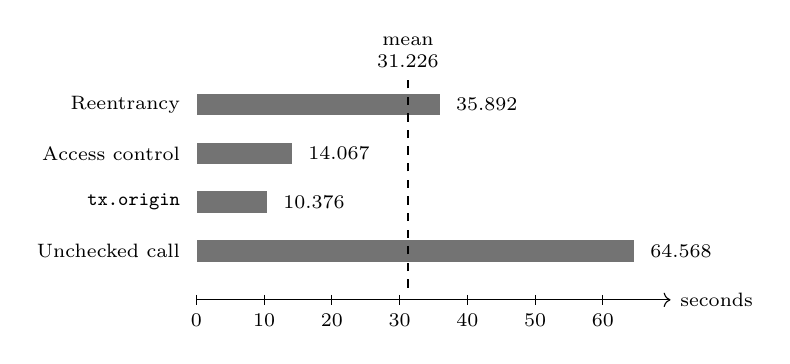
\begin{tikzpicture}[x=0.086cm,y=0.62cm,font=\scriptsize]
\draw[->] (0,0)--(70,0) node[right]{seconds};
\foreach \x in {0,10,...,60}{\draw (\x,0.10)--(\x,-0.10) node[below]{\x};}
\foreach \name/\value/\y in {Reentrancy/35.892/4,{Access control}/14.067/3,{\code{tx.origin}}/10.376/2,{Unchecked call}/64.568/1}{
  \fill[black!55] (0,\y-0.22) rectangle (\value,\y+0.22);
  \node[anchor=east] at (-1,\y) {\name};
  \node[anchor=west] at (\value+1,\y) {\value};
}
\draw[dashed,thick] (31.226,0.25)--(31.226,4.55) node[above,align=center]{mean\\31.226};
\end{tikzpicture}
\caption{Measured end-to-end runtime by fixture.}
\label{fig:runtime}
\end{figure}

The result answers RQ2 for the four templates and RQ3 only for their specified tests: exploit generation and validated repair rates were both 100\%, compilation and regression preservation were 4/4, and the mean retry count was zero. It does not answer whether retries improve repair because no fixture triggered the loop. Patch size was retained in each unified diff but was not aggregated by the experiment report.

Table~\ref{tab:metricstatus} distinguishes measured outcomes from metrics that the present evidence cannot support. Precision is $TP/(TP+FP)$, recall is $TP/(TP+FN)$, F1 is $2PR/(P+R)$, and false-positive rate is $FP/(FP+TN)$. Reporting a guessed value for any unavailable cell would convert a missing experiment into fabricated evidence.

\begin{table}[t]
\caption{Metric status for the reported experiment}
\label{tab:metricstatus}
\centering\footnotesize
\begin{tabularx}{\columnwidth}{@{}p{2.0cm}p{1.25cm}Y@{}}
\toprule
Metric & Value & Evidential basis\\
\midrule
PoC success & 100\% & 4/4 known vulnerable fixtures\\
Validated repair & 100\% & 4/4 confirmed exploits\\
Build/regression & 100\% & 4/4 accepted repairs\\
Mean runtime & 31.226 s & Four completed runs\\
Mean retries & 0 & No fixture required retry\\
Precision/recall/F1 & N/A & Zero coverage-complete labeled cases\\
False-positive rate & N/A & No reviewed clean controls\\
Gas and token cost & N/A & Not aggregated; no API-funded model\\
\bottomrule
\end{tabularx}
\end{table}

\subsection{Coverage Failure and Metric Boundary}
Mythril completed its configured source analysis in all four cases, while Slither failed in all four. Consequently, the experiment marked all four labeled cases as coverage-incomplete and admitted zero cases to the detection-metric denominator. Precision, recall, F1, and false-positive rate are therefore unavailable. The fixture heuristic still selected the known candidate, which allowed the downstream Forge and repair gates to execute; counting that selection as analyzer accuracy would leak the expected solution into the measurement.

The repository also contains a deterministic 500-project Solidity-0.8 subset of FORGE with 3,092 audit-derived finding records~\cite{forgeartifacts}. The current FORGE runner measures bounded Slither case-level coverage and explicitly withholds precision because the manifest is audit-positive and lacks clean controls. A defensible next experiment must report the flow from 500 projects to buildable projects, completed analyzer runs, location-matched ground truth, confirmed exploits, generated patches, and validated repairs. Until that run and manual matching are completed, the manifest is dataset material rather than a performance result.

\subsection{Baseline and Ablation Status}
The executable profiles provide the requested baselines and ablations: Slither, Mythril, their union, confirmation without Red Team, one repair attempt, and the full bounded loop. This revision does not report comparisons among those profiles because incomplete Slither execution would make the budgets and denominators unequal. RQ1 and RQ4 therefore remain unanswered. A held-out study must run every profile on identical source revisions and time budgets, include clean controls, repeat stochastic model paths, and report vulnerability-wise failures as well as successes.

Table~\ref{tab:comparison} places the fixture result beside published systems. The tasks, datasets, models, and success oracles differ, so these values provide context rather than a ranking. In particular, Sentinel's 4/4 result is template-assisted engineering evidence and cannot establish superiority over results on held-out or real-world contracts.

\begin{table*}[t]
\caption{Contextual comparison with published exploit-generation and repair systems}
\label{tab:comparison}
\centering\footnotesize
\begin{tabularx}{\textwidth}{@{}p{2.15cm}p{2.55cm}p{4.25cm}Y@{}}
\toprule
System & Primary task & Evaluation scope & Published or measured result\\
\midrule
Prompt to Pwn (ReX)~\cite{prompttopwn} & Exploit generation & Synthetic and real-world benchmarks; five LLMs & Up to 92\% exploit-generation success\\
PoCo~\cite{poco} & Exploit generation & 23 real-world vulnerability reports & Generates executable Foundry PoCs; the abstract does not state one aggregate success rate\\
ContractTinker~\cite{contracttinker} & Vulnerability repair & 48 high-risk real-world vulnerabilities & 23 valid patches (48\%); 10 more (21\%) required minor changes\\
SCPatcher~\cite{scpatcher} & Vulnerability repair & Vulnerable contracts supported by a 5,000-contract knowledge graph & 81.5\% repair rate and 91.0\% compilation pass rate\\
Sentinel (this work) & Confirmation plus repair & Four known, template-supported Foundry fixtures & 4/4 PoCs and 4/4 validated repairs; detection coverage incomplete\\
\bottomrule
\end{tabularx}
\end{table*}

\section{Limitations and Engineering Implications}
\subsection{Oracle Strength and Generalization}
The principal construct threat is the gap between operational acceptance and semantic correctness. A passing generated test may assert the wrong impact, while a failed exploit after patching may result from disabled functionality. Existing regression tests may omit required behavior, and selecting one candidate leaves other warnings untouched. The internal-validity threat is solution leakage from the four known templates. External validity is limited by the absence of held-out and clean contracts. Reproducibility is limited by tool availability and by unrecorded CPU, RAM, prompt-token, patch-size, and gas aggregates. An accepted fixture patch is therefore evidence for its specified scenario, not a statement that the project is secure.

The fixture benchmark used real Forge execution, but its templates encode known solutions. Its 4/4 result measures implementation behavior rather than discovery or repair of unseen vulnerabilities. Slither's four failures also prevent a fair full-coverage detection comparison. Static inventory of a 500-project manifest does not imply successful compilation or analysis of 500 projects, and the existing case-level FORGE runner does not yet match each warning to an audited type and location.

\subsection{Isolation and Patch Integrity}
Workspace copying is useful for preserving original sources but does not contain malicious build configuration. The runner inherits the host environment, and allowlisted tools may expose capabilities beyond the specific commands used by the workflow. Running untrusted projects would require operating-system isolation, restricted credentials and network access, and careful control of test-engine features. The prototype's local defensive intent is therefore an operating assumption, not a proven containment boundary.

The generic diff path also needs stronger transactional guarantees. It applies allowed-file changes before checking that the returned target list contains only the candidate file. Its failure handler restores the candidate source but does not implement complete rollback for every previously touched file. A hardened version should validate all targets first, stage edits in a disposable copy, and atomically accept only a fully validated single-file result. Prompt-level requests to preserve tests and ABI should become independently checked invariants.

Retry history creates useful diagnostic evidence, but it does not by itself improve generated repairs. Effective correction needs explicit Validator feedback in later patch prompts, a clear difference between model-provider failures and validation failures, and reliable restoration of source files after every rejected attempt. These changes remain future work.

\section{Conclusion}
Sentinel demonstrates a practical and reviewable direction for smart-contract remediation: it connects analyzer evidence, executable attacks, constrained source changes, and deterministic acceptance gates in one local workflow. Its strongest contribution is this closed evidence chain. Unlike a detector-only report or an unvalidated model suggestion, a Sentinel decision preserves the candidate's provenance, the executable exploit, the exact patch, the replay result, regression output, and retry history. This makes the prototype useful both as a developer tool and as an experimental platform for studying where automated security repair succeeds or abstains.

The implementation evidence is encouraging. All 82 automated tests passed, and every one of the four known fixtures produced a confirmed exploit and a repair that passed compilation, exploit-defense, and regression gates with zero retries. The architecture also combines capabilities that prior systems often evaluate separately: analyzer-driven discovery, Foundry-based exploit confirmation, guarded repair application, and closed-loop validation. The comparison table does not establish numerical superiority because its studies use different datasets and oracles, but it highlights Sentinel's distinctive end-to-end integration and transparent state ledger.

The current limitations define a clear evaluation path rather than weakening the engineering contribution. Completing matched FORGE runs, clean-control baselines, profile ablations, independent behavioral oracles, and failure analysis will permit valid precision, recall, F1, and false-positive measurements. With those additions, Sentinel can mature from a successful fixture-backed prototype into a reproducible benchmark platform for evidence-guided smart-contract security assessment and repair.

\begin{thebibliography}{99}
\bibitem{poco} V. Andersson \emph{et al.}, ``PoCo: Agentic proof-of-concept exploit generation for smart contracts,'' arXiv:2511.02780, 2025--2026. [Online]. Available: \url{https://arxiv.org/abs/2511.02780}.
\bibitem{slither} J. Feist, G. Grieco, and A. Groce, ``Slither: A static analysis framework for smart contracts,'' arXiv:1908.09878, 2019. [Online]. Available: \url{https://arxiv.org/abs/1908.09878}.
\bibitem{mpro} ``MPro: Combining static and symbolic analysis for scalable testing of smart contracts,'' arXiv:1911.00570, 2019. [Online]. Available: \url{https://arxiv.org/abs/1911.00570}.
\bibitem{echidna} G. Grieco, W. Song, A. Cygan, J. Feist, and A. Groce, ``Echidna: Effective, usable, and fast fuzzing for smart contracts,'' in \emph{Proc. ISSTA}, 2020, doi: 10.1145/3395363.3404366.
\bibitem{fuzzordering} Z. Liu, P. Qian, Q. He, \emph{et al.}, ``Rethinking smart contract fuzzing: Fuzzing with invocation ordering and important branch revisiting,'' arXiv:2301.03943, 2023. [Online]. Available: \url{https://arxiv.org/abs/2301.03943}.
\bibitem{prompttopwn} ``Prompt to Pwn: Automated exploit generation for smart contracts,'' arXiv:2508.01371, 2025. [Online]. Available: \url{https://arxiv.org/abs/2508.01371}.
\bibitem{v2e} ``V2E: Validating smart contract vulnerabilities through profit-driven exploit generation and execution,'' arXiv:2604.13611, 2025. [Online]. Available: \url{https://arxiv.org/html/2604.13611}.
\bibitem{contracttinker} C. Wang, J. Zhang, \emph{et al.}, ``ContractTinker: LLM-empowered vulnerability repair for real-world smart contracts,'' in \emph{Proc. ASE}, 2024, doi: 10.1145/3691620.3695349.
\bibitem{scpatcher} ``SCPatcher: Automated smart contract code repair via retrieval-augmented generation and knowledge graph,'' arXiv:2604.00687, 2026. [Online]. Available: \url{https://arxiv.org/abs/2604.00687}.
\bibitem{smartfix} S. So and H. Oh, ``SmartFix: Fixing vulnerable smart contracts by accelerating generate-and-verify repair using statistical models,'' in \emph{Proc. ESEC/FSE}, 2023, pp. 185--197, doi: 10.1145/3611643.3616341.
\bibitem{mitigation} S. Bobadilla, M. Jin, and M. Monperrus, ``Do automated fixes truly mitigate smart contract exploits?'' arXiv:2501.04600, 2025. [Online]. Available: \url{https://arxiv.org/abs/2501.04600}.
\bibitem{multise} ``LLM-based multi-agent systems for software engineering: Literature review, vision and the road ahead,'' arXiv:2404.04834, 2024--2025. [Online]. Available: \url{https://arxiv.org/abs/2404.04834}.
\bibitem{llm4vuln} ``LLM4Vuln: A unified evaluation framework for decoupling and enhancing LLMs' vulnerability reasoning,'' arXiv:2401.16185, 2024. [Online]. Available: \url{https://arxiv.org/abs/2401.16185}.
\bibitem{smartbugs} J. F. Ferreira, P. Cruz, T. Durieux, and R. Abreu, ``SmartBugs: A framework to analyze Solidity smart contracts,'' in \emph{Proc. ASE}, 2020, pp. 1349--1352, doi: 10.1145/3324884.3415298.
\bibitem{forgeartifacts} J. Chen \emph{et al.}, ``FORGE: An LLM-driven framework for large-scale smart contract vulnerability dataset construction,'' in \emph{Proc. ICSE}, 2026, pp. 491--503, doi: 10.1145/3744916.3764529.
\end{thebibliography}
\end{document}
